\documentclass[conference]{IEEEtran}
\usepackage{graphicx}
\usepackage{booktabs}
\usepackage{amsmath}
\title{FlightReady v2: Evidence-Aware Data Readiness for Intelligent UAV Systems}
\author{\IEEEauthorblockN{Anonymous submission}\IEEEauthorblockA{Double-blind review}}
% Camera-ready identity (activate only after acceptance and author confirmation):
% Aditya Pratap Singh, Undergraduate Researcher, The Pennsylvania State University.
% Department, email, ORCID, and any coauthors remain intentionally unspecified.
% Camera-ready AI-assistance disclosure, subject to IEEE IV 2027 and institutional review:
% OpenAI Codex provided substantive assistance with research software development,
% automated experiment orchestration, analysis scripting, and manuscript preparation.
% The researcher directed the study, verified the retained evidence, and accepts
% responsibility for the manuscript. This disclosure does not resolve the IV 2027
% prohibition on LLM-generated manuscripts; a human-authored rewrite may be required.
\begin{document}
\maketitle
\begin{abstract}I present FlightReady v2, an evidence-aware data-readiness pipeline for intelligent UAV systems. The frozen method retains unavailable evidence in coverage, separates weighted geometric aggregation from readiness gates, and withholds the primary score when applicable evidence is incomplete. All 19 amended-plan runs are complete; two additional valid Gaussian-25 observations are labeled supplemental. Reference-free scores were withheld at 55.6\% coverage. Sensitivity was 10\% reference-free and 100\% with either a deterministic 10\% audit or full oracle. Across eight related condition means, Pearson r=.767 (p=.0263) and Spearman rho=.838 (p=.0093), but these descriptive associations do not independently validate prediction.\end{abstract}
\begin{IEEEkeywords}data readiness, data quality, evidence coverage, UAV, object detection, reproducibility\end{IEEEkeywords}
\section{Introduction}
Machine-learning systems can fail because their training data are incomplete, mislabeled, unrepresentative, or supported by insufficient evidence. Data-quality tools usually report the checks they can compute, but a high partial score can be mistaken for a complete readiness judgment. I developed FlightReady to investigate whether a dataset supplies sufficient quality evidence for a stated intelligent-system task while keeping missing evidence visible.
The project progressed through three empirical stages. A tabular study first exposed a failure mode in FlightReady v1: the score remained 100 at 50\% evidence coverage while regression performance declined. A VisDrone object-detection study then produced a negative, nonsignificant v1 association. I used those design-set results to formulate and freeze FlightReady v2, which separates quality aggregation, evidence coverage, and readiness gates. I subsequently evaluated the frozen method on UAVVaste, an independently sourced UAV dataset not used to design v2.
The research questions are: (RQ1) Does frozen v2 respond to controlled defects in an unfamiliar UAV dataset? (RQ2) Which defects are detectable without trusted reference evidence, with a limited audit, and with a full oracle? (RQ3) How do readiness scores correspond to detector performance under the completed protocol? (RQ4) Which conclusions remain unsupported?
This paper contributes a context-aware evidence model that withholds the primary score when applicable evidence is incomplete; an implementable, frozen aggregation and decision procedure; controlled evidence spanning tabular, VisDrone, and UAVVaste studies; and an explicit negative result that reference-free checks remain inadequate for semantic correctness and acquisition completeness. I do not claim that FlightReady predicts detector accuracy, establishes causal effects, or certifies operational safety.
\section{Related Work}
Data-readiness work treats quality as contextual and connected to downstream use rather than as a context-free dataset property \cite{r1,r2,r3}. Data-cascade research shows that collection and labeling problems propagate through model development [4], while datasheets encourage explicit documentation of composition, provenance, collection, and recommended use [5]. FlightReady complements documentation by producing a task-specific assessment record with metric provenance, unavailable-evidence states, weighted coverage, score bounds, and independent decision gates.
These mechanisms differ from conventional data validation. Schema validity, file readability, duplicates, annotation counts, and simple distribution comparisons are useful baselines, but they cannot establish whether labels are semantically correct or whether acquisition is complete without trusted evidence. FlightReady therefore represents the boundary between measured quality and unknown quality rather than converting unknown evidence into a pass.
VisDrone is a large multi-class UAV object-detection benchmark with small objects, occlusion, viewpoint variation, and clutter \cite{r6}. UAVVaste targets low-altitude aerial litter detection and contains sparse, small instances in a one-class setting \cite{r7,r8}. Its domain and label structure differ from the urban imagery used during the VisDrone design study, making it suitable for a limited independent validation while still representing only one external dataset.
\section{Flightready V2 Methodology}
A. Context and evidence states. A project declares the task, target labels, acquisition assumptions, and applicable metrics. Each applicable metric is measured, unavailable, or not applicable. Unavailable evidence remains in the applicability denominator; it is never converted into a passing value. Each measured metric produces a normalized score q\_i in [0,100], a positive weight w\_i, provenance, and threshold evidence.
B. Weighted geometric aggregation. Let A be the applicable metrics and M be the measured subset. The applicable and measured weight totals are W\_A and W\_M. Evidence coverage is the measured-weight fraction. For positive measured scores, the measured-quality summary is defined by (1). The denominator is the sum of measured weights, not a count of metrics. If any measured score with positive weight is zero, the implementation returns Q\_M=0 directly because the logarithm is undefined and the geometric product contains a zero factor.
\begin{align}W_A&=\sum_{i\in A}w_i, & W_M&=\sum_{i\in M}w_i, & c&=\frac{W_M}{W_A},\\ Q_M&=100\exp\!\left(\frac{1}{W_M}\sum_{i\in M}w_i\ln\frac{q_i}{100}\right).\end{align}
The primary quality score equals Q\_M only when coverage is exactly one; otherwise it is withheld. The measured-quality summary remains available but is labeled as partial evidence. Lower and upper score bounds are computed over A by assigning every unmeasured applicable metric a score of zero or 100, respectively. Consequently, any unmeasured positive-weight metric makes the strict lower geometric bound zero.
C. Independent readiness gates. The fixed decision order is assessment error, measured blocking failure, unknown blocking evidence or coverage below 0.8, measured warning, and ready. A numeric summary therefore cannot override a blocking gate. The primary score requires complete applicable evidence even though the categorical decision uses a minimum coverage threshold. Algorithm 1 states the implementable procedure.
D. Method freeze. Version flightready-v2.0 was frozen before independent result inspection. The integrity audit verified three recorded file hashes directly. The fourth manifest entry is a malformed 63-character string; inserting its omitted hexadecimal character reproduces the exact CRLF file hash, and LF normalization is byte-identical to the research-release Git blob. The original manifest remains unchanged. This is a documented manifest transcription defect, not a source-code or methodological change.
E. Auditability and interpretation. Each exported scorecard retains the task context, methodology version, measured and unavailable metric states, individual weights and scores, coverage, measured-quality summary, primary-score availability, lower and upper bounds, warnings, blocking reasons, and provenance. This record is necessary because identical numeric summaries can have different meanings when their evidence coverage differs. In particular, Q\_M summarizes only M; it is not an estimator of the unmeasured metrics, a calibrated probability of readiness, or a prediction of model accuracy. The categorical decision is likewise an engineering judgment under declared gates rather than a safety certification.
\begin{figure}[t]\small\textbf{Algorithm 1: FlightReady v2 decision procedure}\par Declare context and $A$; measure $M$ while retaining unavailable evidence; compute $c$, $Q_M$, bounds and gates; withhold $Q$ unless $M=A$; export provenance and hashes.\end{figure}
\section{Experimental Methodology}
A. Historical studies and v2 reassessment. The tabular study trained 108 models across 18 controlled conditions, two regressors, and three seeds. Combined degradation reduced mean R-squared from 0.1635 to 0.0573 for histogram gradient boosting and from 0.1567 to 0.0720 for random forest. The VisDrone study used seven YOLO11n conditions and an untouched test-dev split. Clean mAP@0.5:0.95 was 0.03328; wrong-class, incomplete, and combined conditions reached 0.02928, 0.02808, and 0.02820. V2 reassessment reused these preserved outcomes and is method-development evidence rather than independent validation. Table I separates those stages.
B. Independent UAVVaste dataset. UAVVaste contains 772 images and 3,718 audited COCO annotations for one rubbish category, with official 540/116/116 train/validation/test splits \cite{r7,r8}. The downloaded 3.01-GB archive matched the recorded MD5. All generated variants retained byte-identical official test files, and the audit found zero test-byte issues. Exact filename overlap was zero, although inferred source groups crossed all split pairs, which is a leakage threat.
C. Controlled variants. Deterministic training-only variants used seed 20261112: Gaussian noise at 10\%, 25\%, and 40\% prevalence with RGB sigma 25; horizontal 9-pixel motion blur at 25\%; removal of half the boxes in affected images at 10\%, 25\%, and 40\%; normalized center displacement of +0.08 at 25\%; removal of 40\% of training images; a combined 40\% condition; and a repaired control byte/label equivalent to clean. Wrong-class corruption was inapplicable because the dataset has one valid class.
D. Model protocol and run accounting. YOLO11n and YOLOv8n used pretrained Ultralytics weights \cite{r9}, 832-pixel input, batch 32, deterministic execution, patience 10, two workers, and 40 fixed epochs; optimizer=auto selected AdamW. Validation selected the best checkpoint, and the official test set was used only for final evaluation. A 67-epoch coverage control approximately matched optimizer updates. The amended plan contained 19 runs: three clean and three combined seeds, single-seed primary defects, severity checks, one fixed-update control, and one YOLOv8n clean/combined pair. All 19 are complete. Two Gaussian-25 runs at seeds 42 and 93 satisfy the final protocol but predate the amended plan and are reported separately as supplemental observations.
E. Evidence modes, baselines, and statistics. Reference-free assessment used only dataset-internal observations. The limited mode used one deterministic 10\% trusted annotation audit. Full-oracle mode compared all training content with the clean reference. Baselines included schema and label validity, file completeness, unreadable images, exact duplicates, an absolute clarity proxy, annotation/image counts, and center-distribution shifts. A defect was detected when its score decreased by more than 0.1 point or its warning set changed relative to clean. Pearson and Spearman tests use eight related condition means. Two-sided p-values are descriptive; seed t intervals characterize training stochasticity rather than population or dataset-level generalization.
F. Independence and run controls. The v2 definitions, normalizations, weights, thresholds, coverage rule, aggregation, and gate ordering were locked before the UAVVaste results were interpreted. Variant generation changed training content only. The official validation and test images and annotations were retained, and a byte audit reported no test-set changes. Run identifiers encode model, condition, seed, schedule, batch, and worker count; saved JSON records retain detector metrics, elapsed time, checkpoint identity, and protocol metadata. The two supplemental Gaussian-25 runs were not silently absorbed into plan completion: the amended-plan count remains 19, while their valid measurements are used only where the manuscript explicitly labels n=3 as one planned plus two supplemental observations.
\section{Results}
A. Readiness evidence. Table II reports the representative scorecards. Reference-free primary scores were withheld for every UAVVaste condition because evidence coverage was 55.6\%. Their measured summaries remained between 99.48 and 99.85, demonstrating why a partial summary must not be presented as complete readiness. The full-oracle score fell from 99.83 for clean to 86.83 for combined degradation; the deterministic 10\% audit produced 86.43. Figure 5 shows how trusted evidence changes what can be assessed.
B. Defect sensitivity and baselines. Under the prespecified rule, reference-free assessment detected 1/10 controlled defects, while the deterministic 10\% audit and full oracle each detected 10/10. Conventional baselines detected 5/10, mainly annotation-count and file-coverage changes. Figure 2 compares the methods. These sensitivity values measure assessor response to injected defects; they are not true-positive rates for naturally occurring field errors.
C. Detector performance. Table III reports the primary YOLO11n conditions. The three-seed clean mean was 0.4790 mAP@0.5:0.95 (SD 0.0059; 95\% t interval [0.4643, 0.4937]). Combined-40 averaged 0.4452 (SD 0.0044; interval [0.4341, 0.4562]), a matched-seed mean decrease of 7.05\%. Gaussian-25 averaged 0.4747 (SD 0.0024; interval [0.4688, 0.4806]); only seed 17 belongs to the amended 19-run plan, while seeds 42 and 93 are supplemental. The paired Gaussian-25 difference interval [-0.0229, 0.0144] includes zero. Repair reproduced the matching clean seed at 0.4724. Figure 4 displays repeated-seed variability.
D. Severity, update control, and architecture transfer. Gaussian results were 0.4682, 0.4747, and 0.4621 at 10\%, 25\%, and 40\% prevalence; because the 25\% mean includes two supplemental observations, this is not a monotonic replicated dose-response test. Missing-annotation results declined from 0.4687 at 10\% to 0.4467 at 40\%. The 40\% coverage condition reached 0.4459 at fixed epochs and 0.4472 with approximately matched updates, so additional updates did not remove the observed deficit. YOLOv8n decreased from 0.4861 clean to 0.4454 combined (-8.36\%). Table IV and Fig. 3 summarize these descriptive controls.
E. Statistical interpretation. Figure 1 relates full-oracle scores to the eight prespecified YOLO11n condition means. Pearson r=0.767 (p=0.0263) and Spearman rho=0.838 (p=0.0093) are nominally significant at alpha=.05. The tests are not independent predictive validation: conditions are related interventions on one source dataset, n=8 is small, and repaired duplicates clean bytes and labels. Excluding repaired changes Pearson to r=0.740 (p=0.0573), which does not cross .05, while Spearman remains rho=0.857 (p=0.0137). I therefore treat the correlations as descriptive condition-level association rather than calibration, causal evidence, or proof of dataset-to-dataset generalization.
F. Score behavior by evidence mode. The clean reference-free summary was 99.70, but its primary score was unavailable; Gaussian-25 produced an even higher partial summary of 99.85 although the full-oracle and limited-audit scores were 96.77 and 95.81. Box displacement produced full-oracle and audit scores of 93.68 and 97.85, while coverage loss produced 94.32 and 93.52. These differences are expected because a deterministic subset and a complete reference expose different evidence. The combined condition yielded the lowest scores in both trusted-evidence modes (86.83 oracle and 86.43 audit), whereas repaired returned to the clean value of 99.83. The results demonstrate responsiveness under controlled access to trusted evidence; they do not show that one audit sample is an unbiased estimator of the full oracle.
\section{Discussion}
The strongest supported contribution is evidence accounting rather than accuracy forecasting. FlightReady v2 prevents a near-perfect partial-evidence summary from masquerading as a complete readiness result. Trusted references or audits recover sensitivity to image corruption, label omission, box displacement, coverage loss, and combined corruption, but this sensitivity depends on evidence that practitioners may not possess.
The limited audit detected all injected variants under the prespecified rule, yet it was one deterministic sample and should not be generalized to arbitrary audit fractions or sampling schemes. Likewise, conventional checks provide useful low-cost signals but missed Gaussian noise, motion blur, and displaced boxes in this experiment. These comparisons clarify capability boundaries rather than establish universal superiority.
The historical reassessments are method-development evidence. UAVVaste adds an independently sourced domain, but the score-performance analysis still uses controlled conditions from one dataset. The positive association supports a hypothesis that lower readiness accompanies lower detector performance under this protocol. It does not establish a portable readiness-to-mAP function.
The performance controls also separate several alternative explanations without eliminating them. Matching optimizer updates for 40\% coverage improved mAP@0.5:0.95 only from 0.4459 to 0.4472, leaving a 5.32\% deficit relative to the matching clean seed. The YOLOv8n combined result decreased by 8.36\%, which is directionally consistent with YOLO11n, but each YOLOv8n condition has one seed. Repair exactly reproduced clean data and the matching 0.4724 detector outcome, supporting pipeline determinism for that control rather than proving determinism for every training run.
Practically, FlightReady should be read as a structured argument about evidence sufficiency. A practitioner can inspect which criteria were applicable, why a measurement was unavailable, whether a gate failed, and how much weight was actually measured. When trusted references are absent, the correct output may be insufficient evidence even when every available technical check passes. That behavior is a substantive result of the project, not a missing implementation feature.
\section{Limitations And Threats To Validity}
External validity is limited to one independently sourced, single-class UAV dataset and two related YOLO detector families. Independent wrong-class validation remains unavailable. The official image-level split contains inferred filename source groups across split pairs, which may include adjacent frames and inflate detector performance. I retained the official split because stronger grouping metadata were unavailable.
Construct validity is limited by the evidence modes. Full-oracle comparison is experimentally informative but operationally unrealistic. The deterministic 10\% audit was not replicated. Gaussian noise can increase a Laplacian sharpness proxy, showing that absolute proxies are content-sensitive. Conventional baselines and FlightReady do not have identical evidence access, so sensitivity comparisons describe practical detection capability rather than a controlled algorithm contest.
Statistical validity is limited by single-seed defect conditions, two supplemental Gaussian observations outside the amended plan, related condition means, and small n. Confidence intervals with three seeds describe training variability only. Metric weights and thresholds are engineering judgments rather than learned utilities. No result implies causal prediction, dataset-level generalization, aviation safety, or certified operational readiness.
Reproducibility is also bounded by the retained software and hardware environment. Pretrained weights and saved checkpoints are identified in the experiment records, but future library, driver, or accelerator changes can affect exact training trajectories. The frozen source identity is recoverable despite the documented 63-character manifest transcription defect, yet the defect itself shows why manifests should be machine-validated at freeze time. The read-only verification script checks the saved evidence; it does not recreate raw training computation from first principles.
\section{Conclusion}
I developed and evaluated FlightReady v2 as a context-aware, evidence-aware readiness pipeline. The 19 completed amended-plan runs, two separately labeled supplemental observations, historical studies, and v2 reassessments support transparent score withholding and reference-assisted controlled-defect sensitivity. They do not establish universal prediction of downstream performance. I conclude that FlightReady v2 is most defensible as an auditable decision-support framework that exposes what is measured, what is missing, and which gates prevent a readiness claim.
\section{Reproducibility}
The artifact package contains the frozen-method manifest, experiment configuration, dataset audit, protocol amendments, per-run JSON records, model checkpoint hashes, scorecards, analysis outputs, and figure-generation inputs. An independent read-only verification recalculated run accounting, group means, paired changes, t intervals, correlations, evidence coverage, geometric scores, categorical decisions, detection sensitivity, and baseline detection from the saved artifacts. The original manifest is preserved with its documented 63-character transcription defect.
The verification succeeded for all 19 planned tags and identified exactly the two declared supplemental tags. Every saved condition-summary value, three-seed interval, paired change, correlation coefficient and p-value, representative scorecard, detection count, and conventional-baseline result matched the independent recalculation. These checks establish internal consistency between the retained artifacts and this manuscript; they do not replace replication on another independently sourced dataset.
\begin{table*}[t]
\caption{Development and validation evidence.}
\centering\scriptsize
\begin{tabular}{p{0.13\textwidth}p{0.19\textwidth}p{0.28\textwidth}p{0.27\textwidth}}
\toprule Study & Scope & Readiness-performance result & Interpretation \\\midrule
Tabular v1 & 108 models; 18 conditions & Score constant 100 at 50\% coverage & Correlation undefined \\
VisDrone v1 & 7 YOLO11n runs & r=-0.377, p=.405 & No supported association \\
Tabular v2 reassessment & Preserved design-set results & r=.790, p=.000096 & Method-development evidence \\
VisDrone v2 reassessment & Preserved design-set results & r=.870, p=.0108 & Method-development evidence \\
UAVVaste v2 & 19 planned + 2 supplemental & r=.767, p=.0263; rho=.838, p=.0093 & Descriptive; not predictive validation \\
\bottomrule\end{tabular}
\end{table*}
\begin{table}[t]
\caption{FlightReady evidence results.}
\centering\scriptsize
\begin{tabular}{lccccc}\toprule Condition & RF & Coverage & Oracle & Audit & Decision \\\midrule
Clean & withheld & 55.6\% & 99.83 & 99.83 & Ready \\
Gaussian 25\% & withheld & 55.6\% & 96.77 & 95.81 & Conditional \\
Blur 25\% & withheld & 55.6\% & 96.57 & 95.89 & Conditional \\
Missing 25\% & withheld & 55.6\% & 98.34 & 98.41 & Conditional \\
Box shift 25\% & withheld & 55.6\% & 93.68 & 97.85 & Conditional \\
Coverage -40\% & withheld & 55.6\% & 94.32 & 93.52 & Conditional \\
Combined 40\% & withheld & 55.6\% & 86.83 & 86.43 & Conditional \\
Repaired & withheld & 55.6\% & 99.83 & 99.83 & Ready \\
\bottomrule\end{tabular}
\end{table}
\begin{table}[t]
\caption{Primary YOLO11n results.}
\centering\scriptsize
\begin{tabular}{lcccc}\toprule Condition & $n$ & mAP50-95 & SD & Relative change \\\midrule
Clean & 3 & 0.4790 & 0.0059 & baseline \\
Gaussian 25\%* & 3 & 0.4747 & 0.0024 & -0.88\% \\
Blur 25\% & 1 & 0.4708 & - & -0.33\% \\
Missing 25\% & 1 & 0.4569 & - & -3.27\% \\
Box shift 25\% & 1 & 0.4533 & - & -4.03\% \\
Coverage -40\% & 1 & 0.4459 & - & -5.61\% \\
Combined 40\% & 3 & 0.4452 & 0.0044 & -7.05\% \\
Repaired & 1 & 0.4724 & - & 0.00\% \\
\bottomrule\end{tabular}
\par\vspace{1mm}\raggedright\scriptsize *Gaussian-25 $n=3$ contains one amended-plan run and two supplemental observations.
\end{table}
\begin{figure}[t]\centering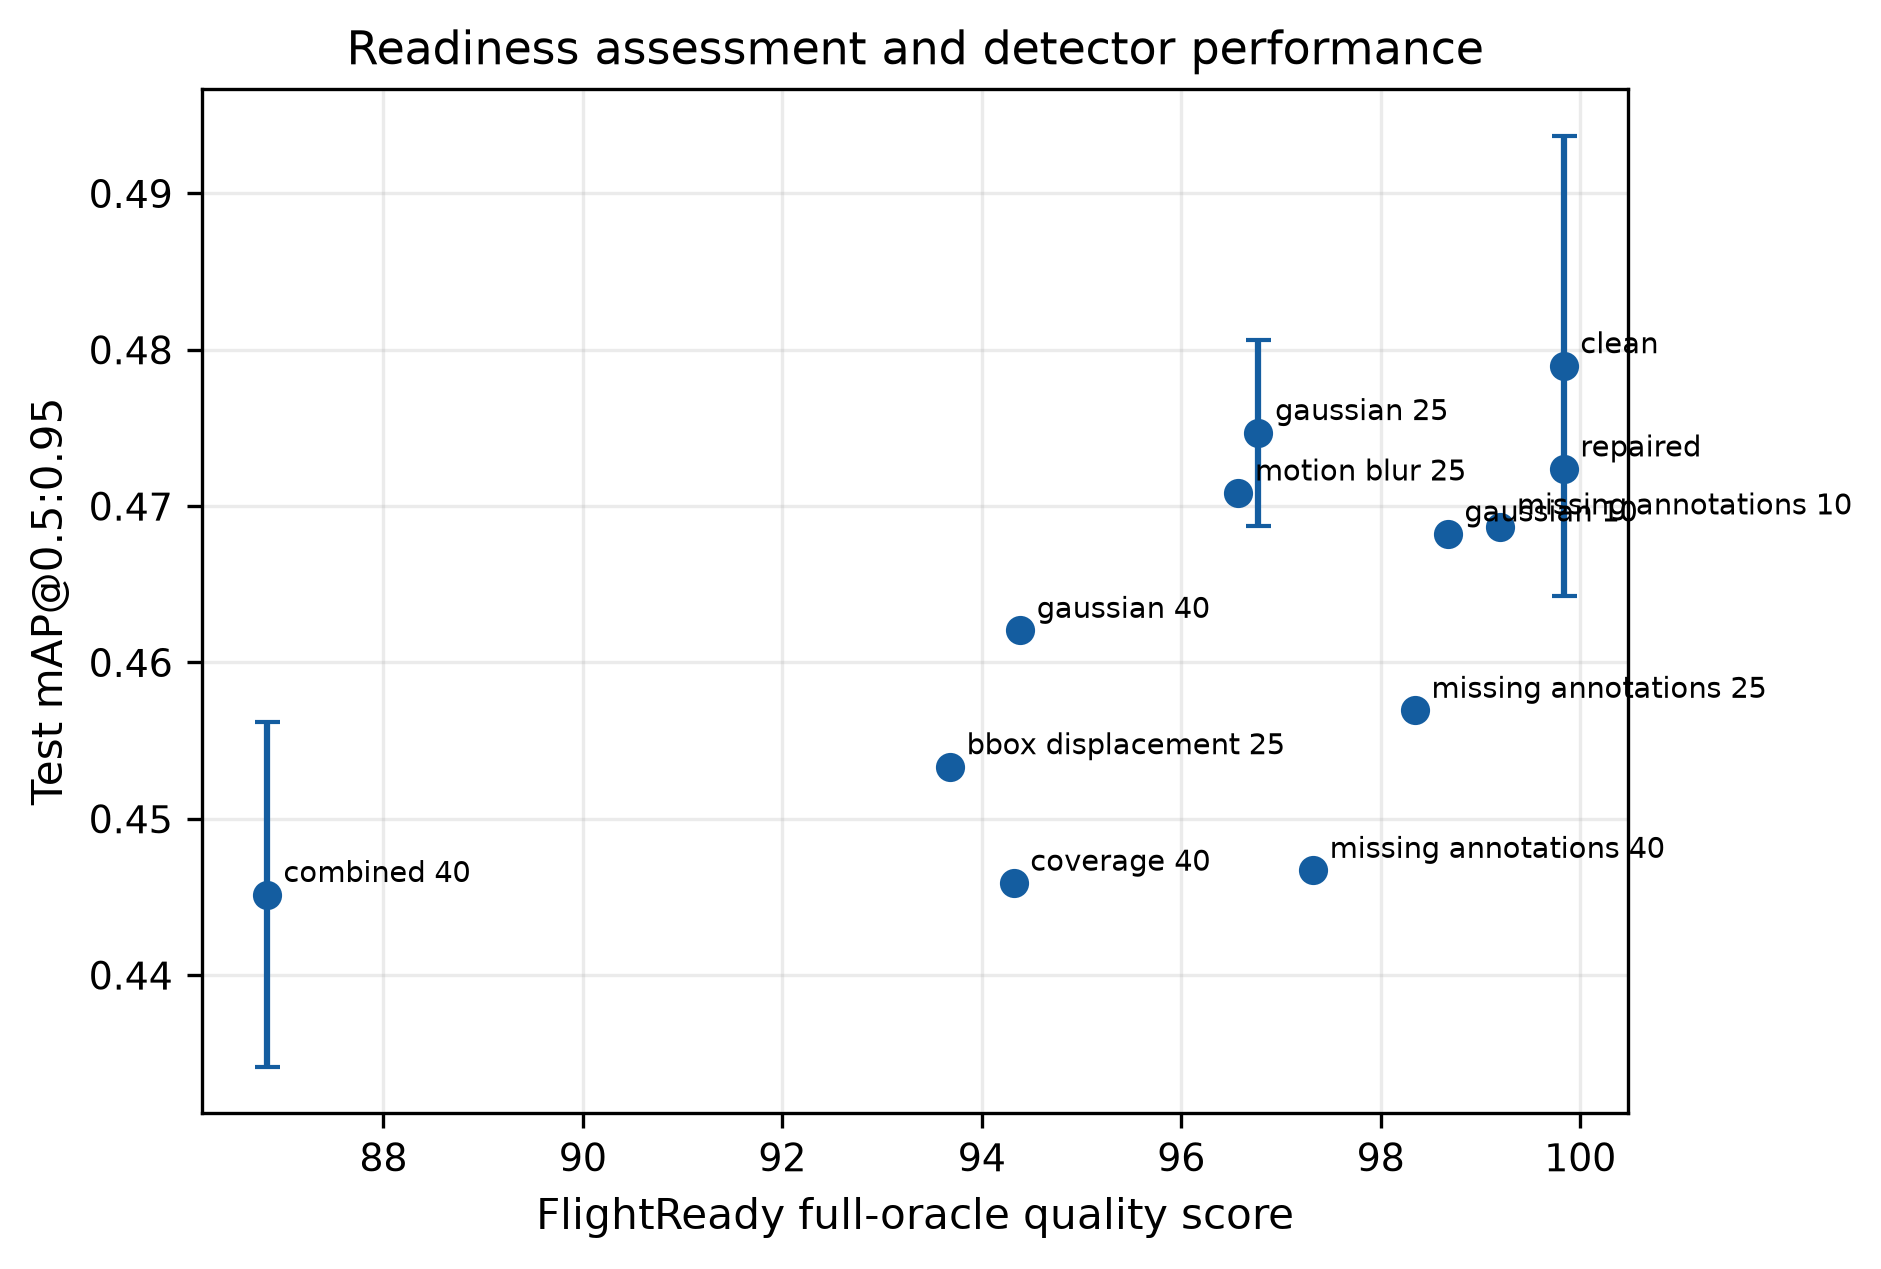
\includegraphics[width=\columnwidth]{figures/01_readiness_vs_performance.png}\caption{Full-oracle score versus condition-mean performance. The relationship is descriptive, not independently validated prediction.}\end{figure}
\begin{figure}[t]\centering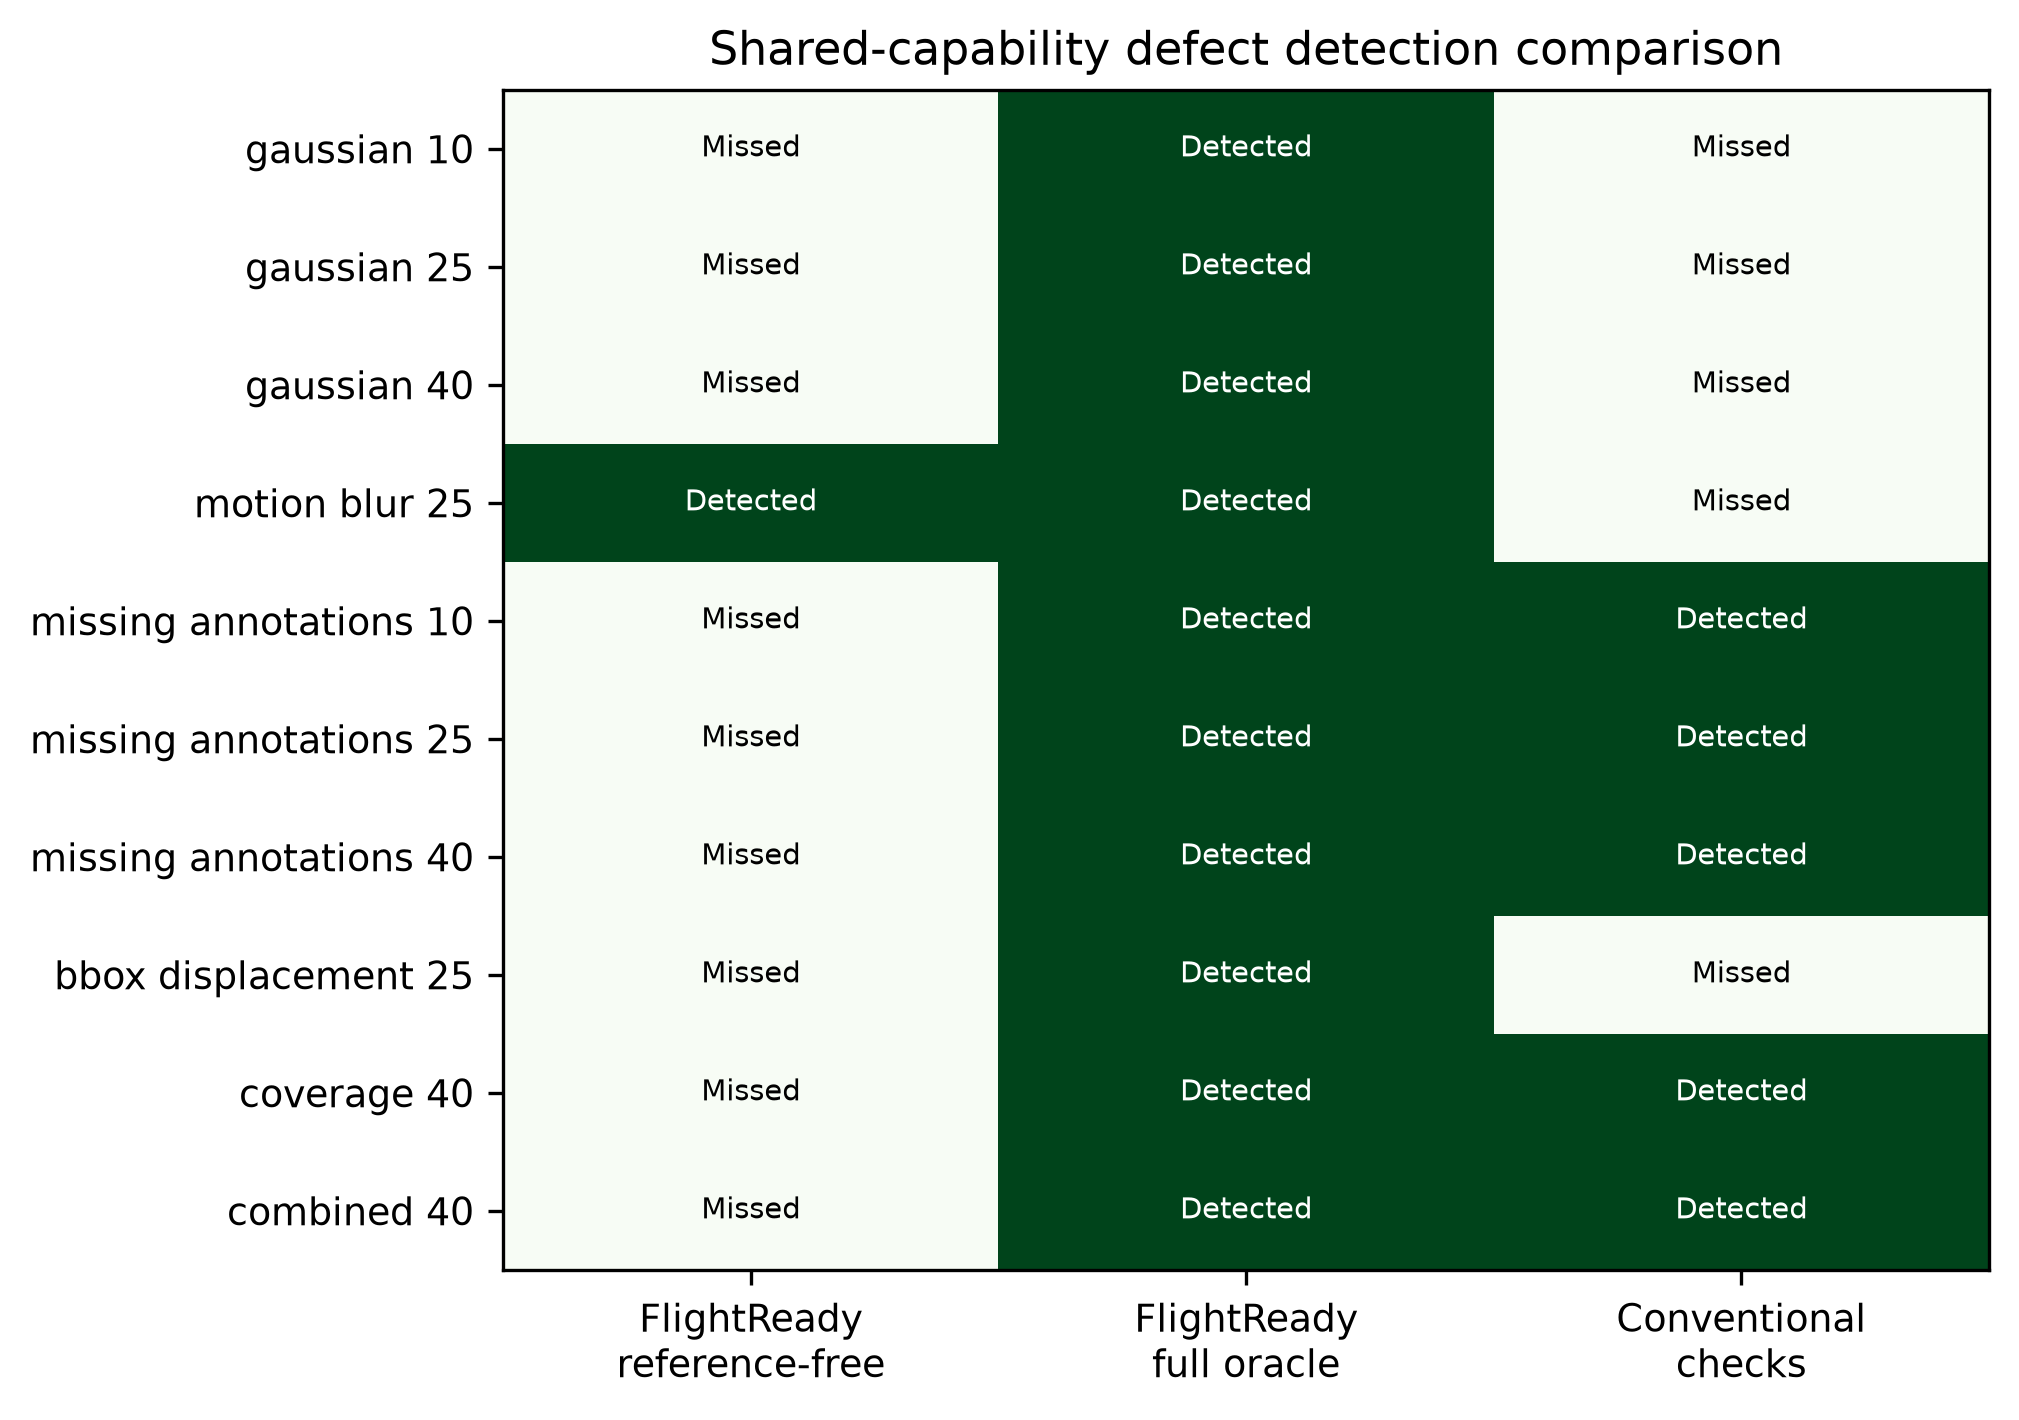
\includegraphics[width=\columnwidth]{figures/07_method_detection_comparison.png}\caption{Controlled-defect detection by evidence mode and conventional baselines.}\end{figure}
\begin{figure}[t]\centering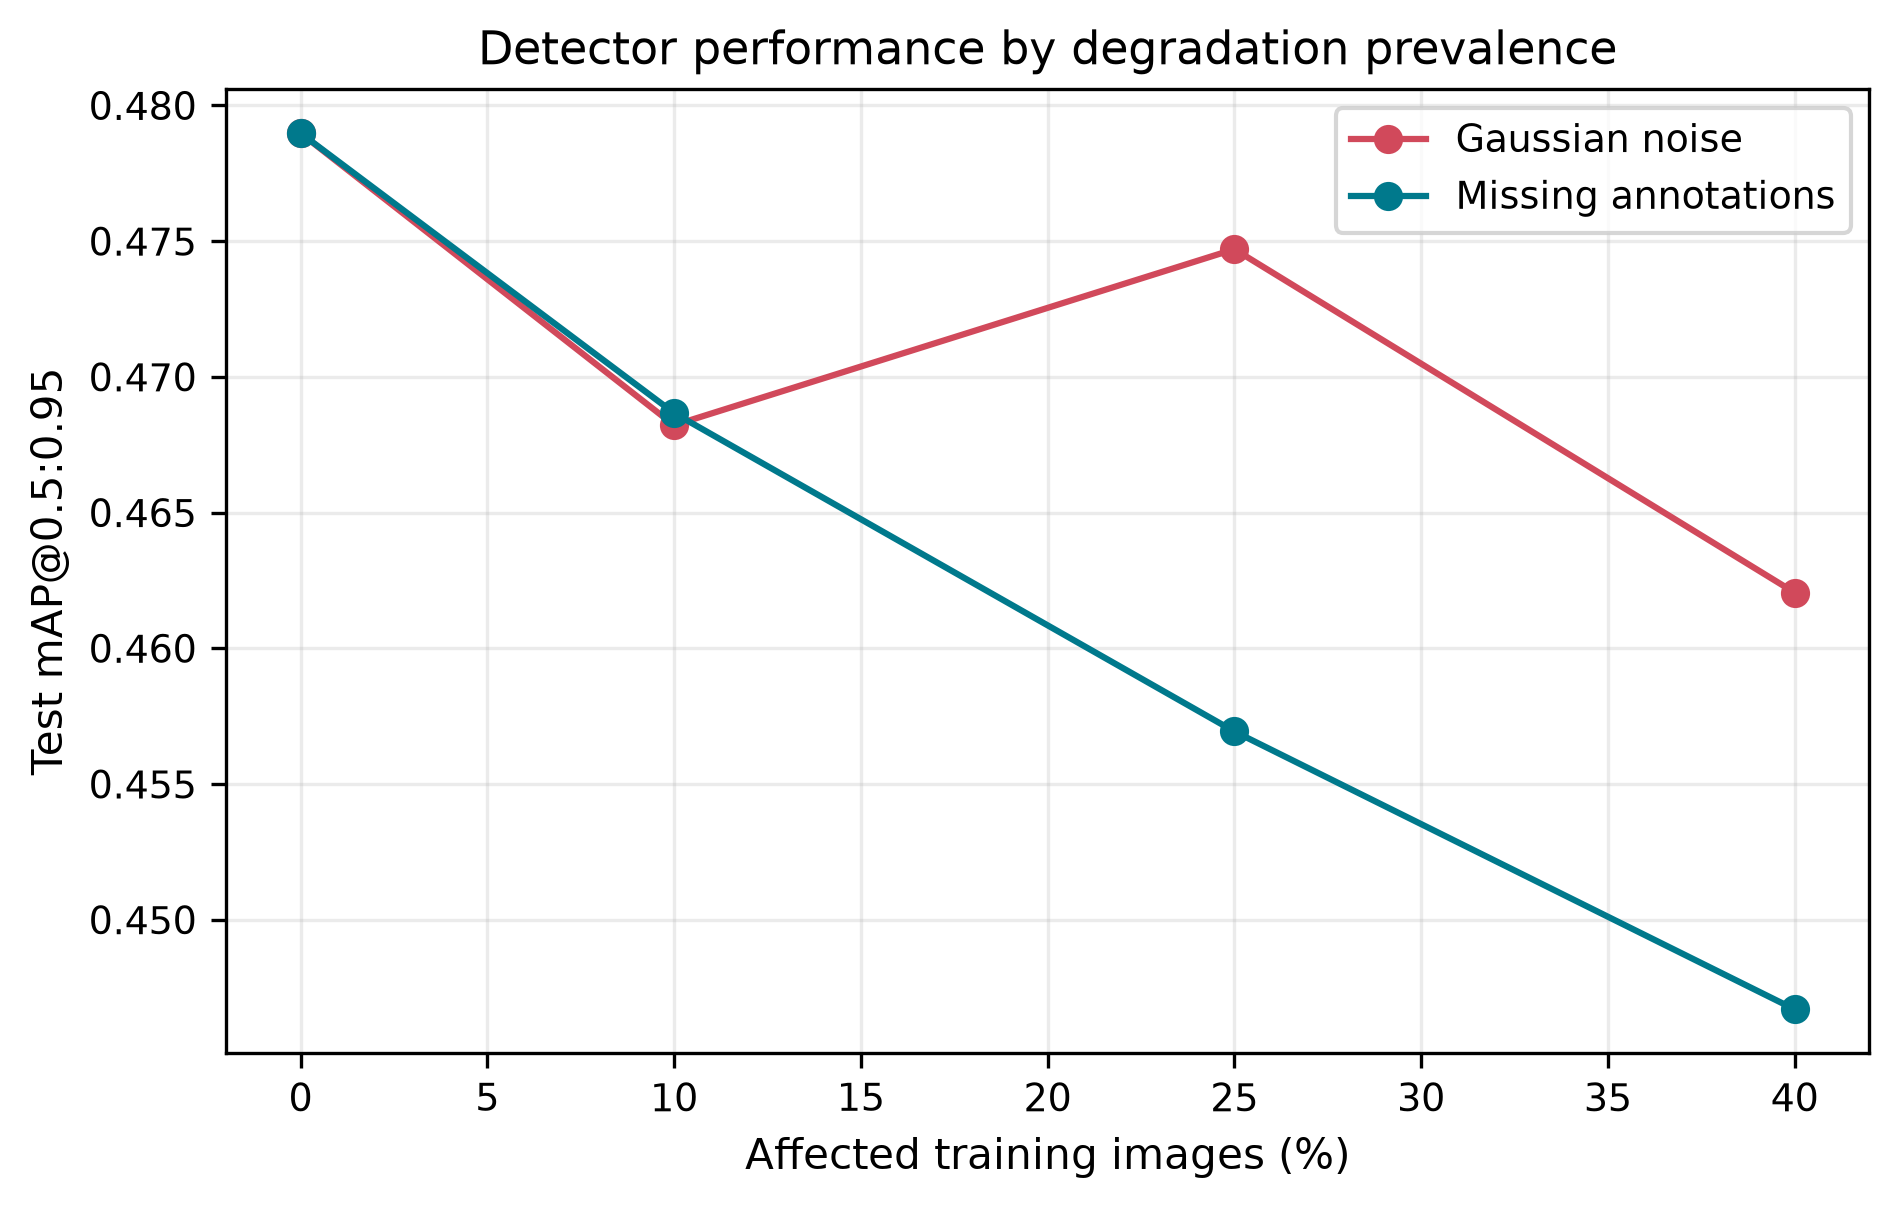
\includegraphics[width=\columnwidth]{figures/02_performance_vs_severity.png}\caption{Single-seed severity observations for Gaussian and missing-annotation variants.}\end{figure}
\begin{table}[t]
\caption{Controls and architecture transfer.}
\centering\scriptsize
\begin{tabular}{lccc}\toprule Comparison & Reference & Result & Change/interpretation \\\midrule
YOLO11n combined, 3 seeds & 0.4790 & 0.4452 & -7.05\% \\
Coverage 40\%, fixed updates & 0.4724 & 0.4472 & -5.32\% \\
YOLOv8n combined, seed 17 & 0.4861 & 0.4454 & -8.36\% \\
Gaussian 10\% -> 40\% & 0.4682 & 0.4621 & severity trend \\
Missing 10\% -> 40\% & 0.4687 & 0.4467 & severity trend \\
\bottomrule\end{tabular}
\end{table}
\begin{figure}[t]\centering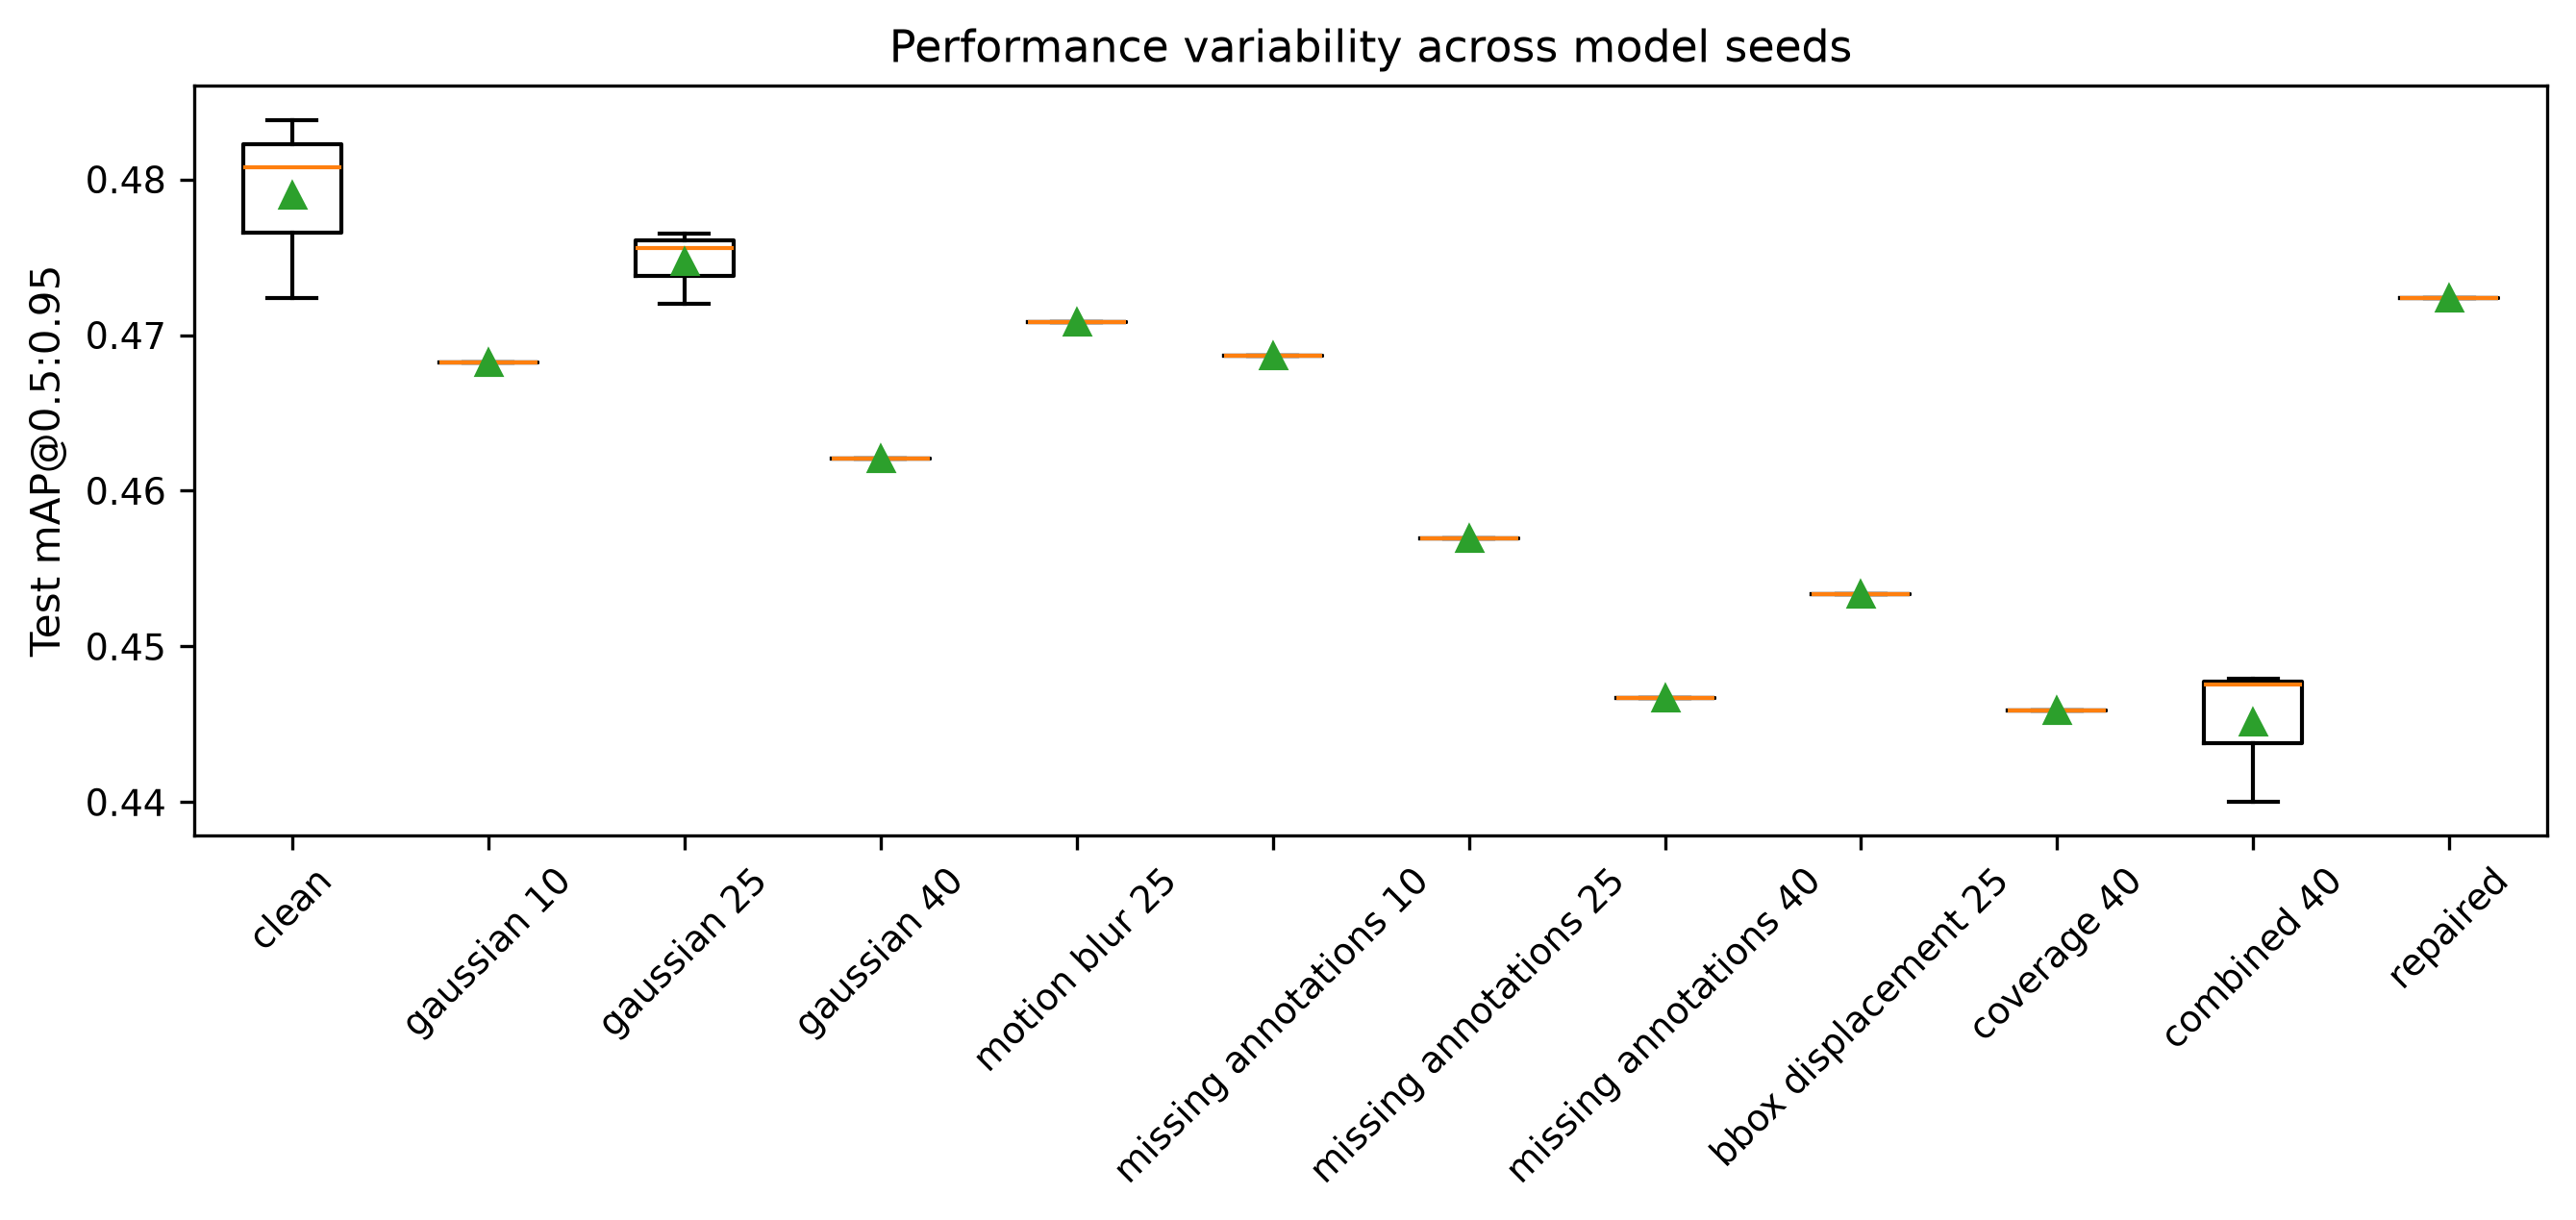
\includegraphics[width=\columnwidth]{figures/08_seed_variability.png}\caption{Seed variability for repeated observations; Gaussian-25 includes two supplemental seeds.}\end{figure}
\begin{figure}[t]\centering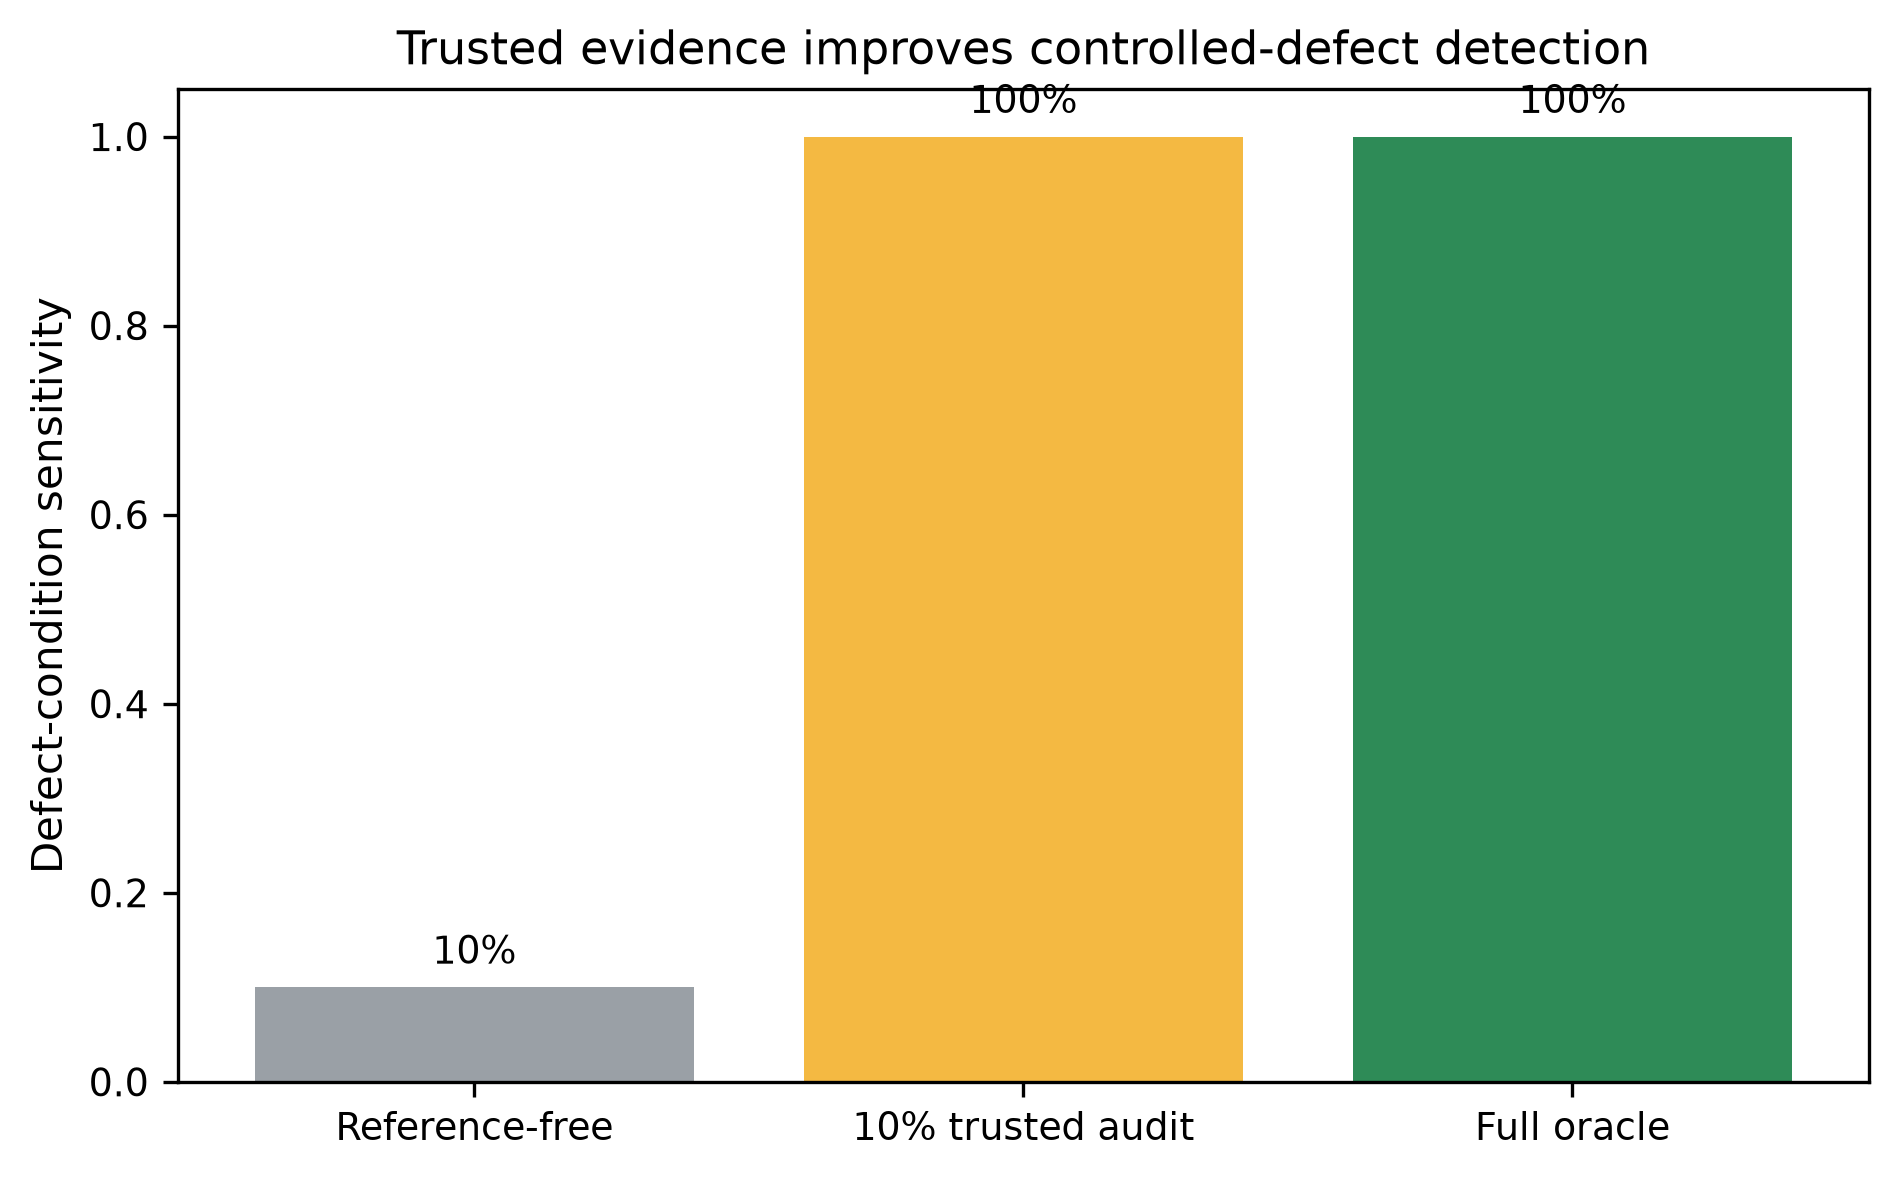
\includegraphics[width=\columnwidth]{figures/04_reference_evidence_detection.png}\caption{Controlled-defect detection changes with trusted reference evidence.}\end{figure}
\begin{thebibliography}{10}
\bibitem{r1} S. Afzal, R. C., M. Kesarwani, S. Mehta, and H. Patel, "Data Readiness Report," arXiv:2010.07213, 2020.
\bibitem{r2} M. Priestley, F. O'Donnell, and E. Simperl, "A Survey of Data Quality Requirements That Matter in ML Development Pipelines," J. Data Inf. Quality, vol. 15, no. 2, pp. 1-39, 2023, doi: 10.1145/3592616.
\bibitem{r3} Y. Gong, G. Liu, Y. Xue, R. Li, and L. Meng, "A survey on dataset quality in machine learning," Inf. Softw. Technol., vol. 162, Art. no. 107268, 2023, doi: 10.1016/j.infsof.2023.107268.
\bibitem{r4} N. Sambasivan et al., "Everyone wants to do the model work, not the data work: Data cascades in high-stakes AI," in Proc. CHI, 2021, doi: 10.1145/3411764.3445518.
\bibitem{r5} T. Gebru et al., "Datasheets for datasets," Commun. ACM, vol. 64, no. 12, pp. 86-92, 2021, doi: 10.1145/3458723.
\bibitem{r6} P. Zhu et al., "VisDrone-DET2018: The Vision Meets Drone Object Detection in Image Challenge Results," in Proc. ECCV Workshops, 2018.
\bibitem{r7} M. Kraft et al., "Autonomous, Onboard Vision-Based Trash and Litter Detection in Low Altitude Aerial Images Collected by an Unmanned Aerial Vehicle," Remote Sens., vol. 13, no. 5, Art. no. 965, 2021, doi: 10.3390/rs13050965.
\bibitem{r8} M. Kraft et al., "UAVVaste," Zenodo, 2023, doi: 10.5281/zenodo.8214061.
\bibitem{r9} Ultralytics, "Ultralytics YOLO Documentation." [Online]. Available: https://docs.ultralytics.com/. Accessed: Nov. 13, 2026.
\end{thebibliography}
\end{document}
